%CS6240 Software Engineering project paper

% Ge Gao - Nov. 1, 2009

\documentclass[acmtocl]{acmtrans2m}
\usepackage{graphicx}

%\documentclass[acmtocl]{}
%\documentclass{article}
%\usepackage{times}
\newcommand{\BibTeX}{{\rm B\kern-.05em{\sc i\kern-.025em b}\kern-.08em
    T\kern-.1667em\lower.7ex\hbox{E}\kern-.125emX}}


\begin{document}

% Article top matter
\title{Enabling Go Game on Android Platform} %\LaTeX is a macro for printing the Latex logo
\author{
  Ge Gao, Gu Lin, Michael Skalak\\
Department of Computer Science\\
University of Virginia\\
\texttt{\{gg5j,gl2hv,mss6s\}@virginia.edu}\\
}  %\texttt formats the text to a typewriter style font
\date{}  %\today is replaced with the current date

\maketitle

\begin{abstract}
Human Computer Interaction go game on mobile devices is everywhere today. Our project's "bang for the buck" lies in connecting cell phone users to worldwide go players on the Internet in mobile manner and getting a good weichi assistantship on mobile device. This could not be achieved previously due to the relative isolation of individule cell phones from 3G resources and their limited computing capability, which could be overcomed by recent  achievements in wide coverage of the wireless network and 3G networks, ability of cell phones to acess Internet, and open APIs of cell phone OS. Our project takes advantage of these achievements to upgrade cell phones' game playing environment.
\end{abstract}


\section{System Design}

\subsection{Requirements}

The requirement for this project was simple: allow a user to play go anywhere.  To meet this requirement the obvious choice was a phone as it has a sufficient level of hardware and is eminently portable.  Three user scenarios guided the development of this system.  In the first, a mobile device would act as a stand alone interface allowing two physically present users to play on a single phone.  The idea behind this scenario is that a user may wish to play a game of go in a circumstance where carrying a physical go board is inconvenient or impossible.  For example, the users may wish to play in a car or airplane.  Our second scenario is person playing an automated go program.  The third scenario is playing another person who is not present but also has an appropriate device.  

Taking a risk centered approach, the developers focused on several of the potential problems facing the system.  The first was difficulty in obtaining an appropriate environment to develop and test on the phone.  Ultimately, the best solution was the Android phone, which is an opensource software platform for mobile development. It is a complete stack, including operating system, middleware and applications.  Android is the first joint project of OHA (Open Handset Alliance) and is powered by Linux operating system. Android ADK provides the tools and APIs necessary to develop applications on this paltform using Java programming language.

Android SDK also provides emulator, a virtual mobile device that runs on your computer and allows prototyping and testing android applications without a physical device.  Further, the system makes no distinction between built-in applications and added ones; facilitating easy extension or replacement of the basic applications.  In a similar vein, no boundaries separate programs; every application can use any other.  The development kit was also free; in contrast, a development kit for Apple's iPhone requires a substantial fee.  Furthermore, any developed application must receive approval from the company before putting it on a phone.  

Another great feature of Android is its choice of xml resources for GUI management. In other words, XML can declare UI elements. The primary advantage to declaring your UI in XML enabling to better separation of the presentation of the application from the code that controls its behavior. Furthermore, UI descriptions are external to application code, allowing changes to it without modification of the source code and recompilation. Additionally, declaring the layout in XML simplifies visualization of the structure of your UI, so it's easier to debug problems.Every XML layout file must contain exactly one root element, which must be a View or View Group object.  Once you've defined the root element, you can add additional layout objects or widgets as child elements to gradually build GUI. Each child element in XML is also either a View or ViewGroup object.
Every application consists of independent screens, with every screen representing an activity. Each activity may contain different views and view groups in a hierarchical tree. Visually, the tree with the view groups and layout objects is the trunk and branches and with the view and Widgets as the leaves. The View class serves as the base for subclasses called "widgets," which offer fully implemented UI objects, like text fields and buttons. The ViewGroup class serves as the base for subclasses called "layouts," which offer different kinds of layout architecture, like linear or relative.
Most applications have more than just one screen, with each screen an activity.    The activities communicate with each other by intents. An “intent” is a simple messsage object and is made up a number of pieces of information about an intention to do something.

The choice of Android was not perfect, as at several points the Android environment had unexpected difficulties or holes.  One such problem was in the integration of the Java code with the Android UI support.  For example, the system allows the user to select a board size.  This size must then pass from the activity monitoring the input screen to the Java class representing the go board.  Making the Java class a subclass of Activity solved this problem.  Another issue was the Android screen touch mode.  The screen registers an attempted single click as a very rapid series of multiple touch events.  Thus when a user tried to click a move that resulted in that same move still being legal (i.e. when stones were removed) the system would rapidly play both the desired move and the subsequent undesired move.  Solving this issue was not particularly strenuous, but determining the cause of this problem was nontrivial.  The most difficult was a poorly integrated testing capability which made effective testing very difficult.  Similarly, we were unable to find a way to display standard out, making "hello world" style testing impossible. 

Another risk was the ability of the phone to have the hardware capability to effectively compute reasonable moves in a short period of time.  The original premise was that the computer player would be entirely contained on the phone, allowing play even when the phone was disconnected from a network.  However, some preliminary experiments demonstrated that this approach was infeasible.  Potentially, the issue has as much to do with inefficient coding as with fundamental issues with the setup; however, moving the computation to a separate machine and setting up communication seemed more appropriate rather than making improving the search the primary focus of the project.

\subsection{Specifications}

To satisfy the requirements, we devised specifications for the several parts of the system.  First, it needed a user interface that would allows a user to view a game and manipulate it in several ways: starting a new game of various sizes, accepting and displaying moves, and choosing one of the modes of play.  Behind this interface, the program needed to have an abstract representation of the board, enforce the rules of the game and compute the final score and endgame.  On top of this basic interface, the phone version had to communicate with other devices.  Separate from this setup, the overall project required a rudimentary go playing engine which the phone could then connect too.  

\subsubsection{Display}
In developing the display, a major risk was the possibility that an entire board could not fit on the screen at one time.  To address this concern, the display had no extraneous buttons or instrumentation.  The only object on the display is a board displaying the current position and allowing moves.  All higher level functions (undo, new game, pass) are on a separate menu.This choice allowed the game board to take up as much display as possible, forestalling the need for a scrolling function.  

Since the scenarios require several different modes of operation, the program needed a base screen to select board size and one of three modes: phone only, player vs computer, and player vs player.  After selection the display only has the board and whose turn it is.  To reach other functions, the player must push a separate on-phone button.  The board itself simply shows the position of the pieces and potentially an illegal move (due to ko, discussed later).  On completion of a game, the winner and final score is displayed.  

\subsubsection{Abstract Representation}
The underlying representation of the board had to be on the phone itself so it needed to be relatively simple.  However, this representation does include several reasonably advanced features.  On the simple side, it has a representation of the board itself, keeping track of the current position of pieces.  It also recognizes legal moves and plays them, removing pieces as necessary.  The board also enforces the ko rule, which disallows a repeating position.  The system also required the ability to deal with end game by allowing the players to mark pieces as dead and also to computer the winner.    

An example of a more advanced feature is the undo function, which allows the user to undo an arbitrary number of moves from the game.  The abstract representation provides this ability by keeping a game tree of all reached board positions.  The undo function is only the simplest of abilities that could be added because of this game tree.  Other possibilities would include saving a branching game and displaying a complex of games (e.g. a dictionary of different corner openings).

\subsubsection{Computer Player}

The technique for the go playing engine is a Monte Carlo approach based on upper confidence trees (UCT).  The underlying idea is based on the rather strange property of go that the program can estimate the value of a position by playing a random (or mostly random) game from that position and determining the winner at the end.  Thus the overall strategy of the program is to iteratively start playing games from the current position creating a tree of the space.  To choose each subsequent move the program considers both how many times that move has been played in previous games in the current search and how often a win has resulted from that move.  In general, the program should select moves which have been played infrequently in order to explore the game tree as much as possible, but countering that tendency is a need to explore the moves that worked in the past in order to ascertain their quality through selective exploration. 

An attempt to multithread this search was unsuccessful. The primary issue is with the bottleneck of the toplevel game which must be accessed by each thread both "going down" when starting a game and "coming up" when updating the winning percentages.  A more sophisticated approach of allocating a thread to each toplevel move resulted in a insubstantial improvement.  This issue was likely due to how a UCT search works.  Since it gradually eliminates moves and spends increasingly less computation on them, the search would need a more sophisticated way of allocating threads as each move became more or less "interesting".  

\subsubsection{Communication}
The first difficulty faced by playing go with remote players locating the phones. Obviously the only identification of phones, the phone number, is not feasible in a prototype application. A simple solution is to set up a server which has a fixed visible physical address to pass actions of one player to another.  Curiously, the Android platform does not provide special support for network applications. This decision can be partly traced to its design guideline – including only phone specific utilities in the SDK implementation and leaving otherwise general utilities to Java API. The phone specific utilities refer to features such as making calls, display interaction, location map, etc. , while general utilities include networking. The idea behind this design is to let developers enjoy the ease of transitting from Java developing experience directly to Android platform.

Thus, in the automated playing mode and the separate playing mode, the phone side program firstly initiate network connection and negociate with the remote go engine on various parameters like board size, playing modes. After connection is established and players are matched successfully, every party begin their iteration between sending move and waiting for move from the other party. All these network communication is implemented through traditional Java socket mechanism.

However, in the other aspect it does need special attention to develop network application on Android platform. One key design point is to enforce responsiveness of Android application. In fact, Android guards against applications that feel sluggish, hang or freeze for significant periods, or take too long to process input. So in general there is always one thread constantly maintaining the user interaction, procesing user's input and providing users with information to keep them involved. All time or resource consuming tasks, such as network access, comprehensive computation, database access, I/O block, operate in background threads. Thus, multi-threading as well as thread synchronization and communication are used extensively in our go program. Every time the phone side program is performing network negociation or sending or receving moves through network, we need instantiate a new thread to host the tasks.

\begin{figure*}[t]
 \centering
 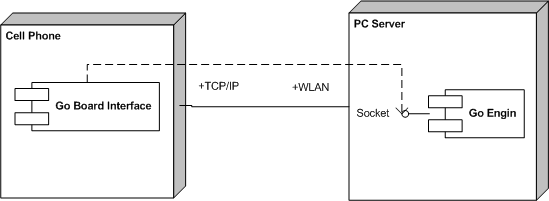
\includegraphics[width = \linewidth]{fig/deployment}
 % deployment.jpg: 549x201 pixel, 96dpi, 14.53x5.32 cm, bb=0 0 412 151
 \label{fig:deploy}
\end{figure*}

\begin{figure*}[t]
 \centering
 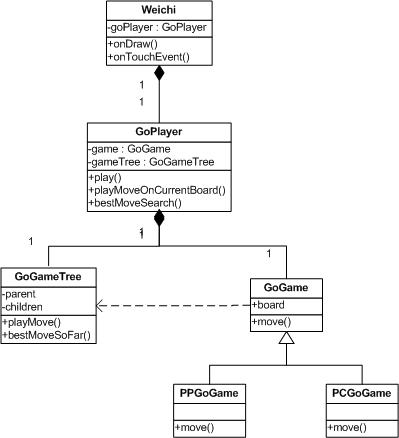
\includegraphics[width = \linewidth]{fig/class}
 % class.jpg: 399x438 pixel, 96dpi, 10.56x11.59 cm, bb=0 0 299 329
 \label{fig:class}
\end{figure*}


\section{Conclusion}
This paper describes the process of creating an environment to play go on an Android phone.  While this program successfully address several risks involved with a full-scale published application.  First, the search and matching ability of phone-to-phone games would need to be adjusted to not only match many different players simultaneously, but also take into consideration relative strengths of the players.   Another way to branch out would be to take advantage of experienced gained in this particular game and apply that to developing a suite of games for mobile devices.   Improving the computer program in both its speed and space requirements so that it plays directly on the phone would be a very useful addition, but potentially the most difficult. 


\end{document}  %End of document.
